\documentclass[tikz,border=6pt]{standalone}
\usepackage[T1]{fontenc}
\usepackage{tikz}
\usetikzlibrary{arrows.meta, positioning, shapes.geometric}
\hyphenpenalty=10000
\exhyphenpenalty=10000

\begin{document}
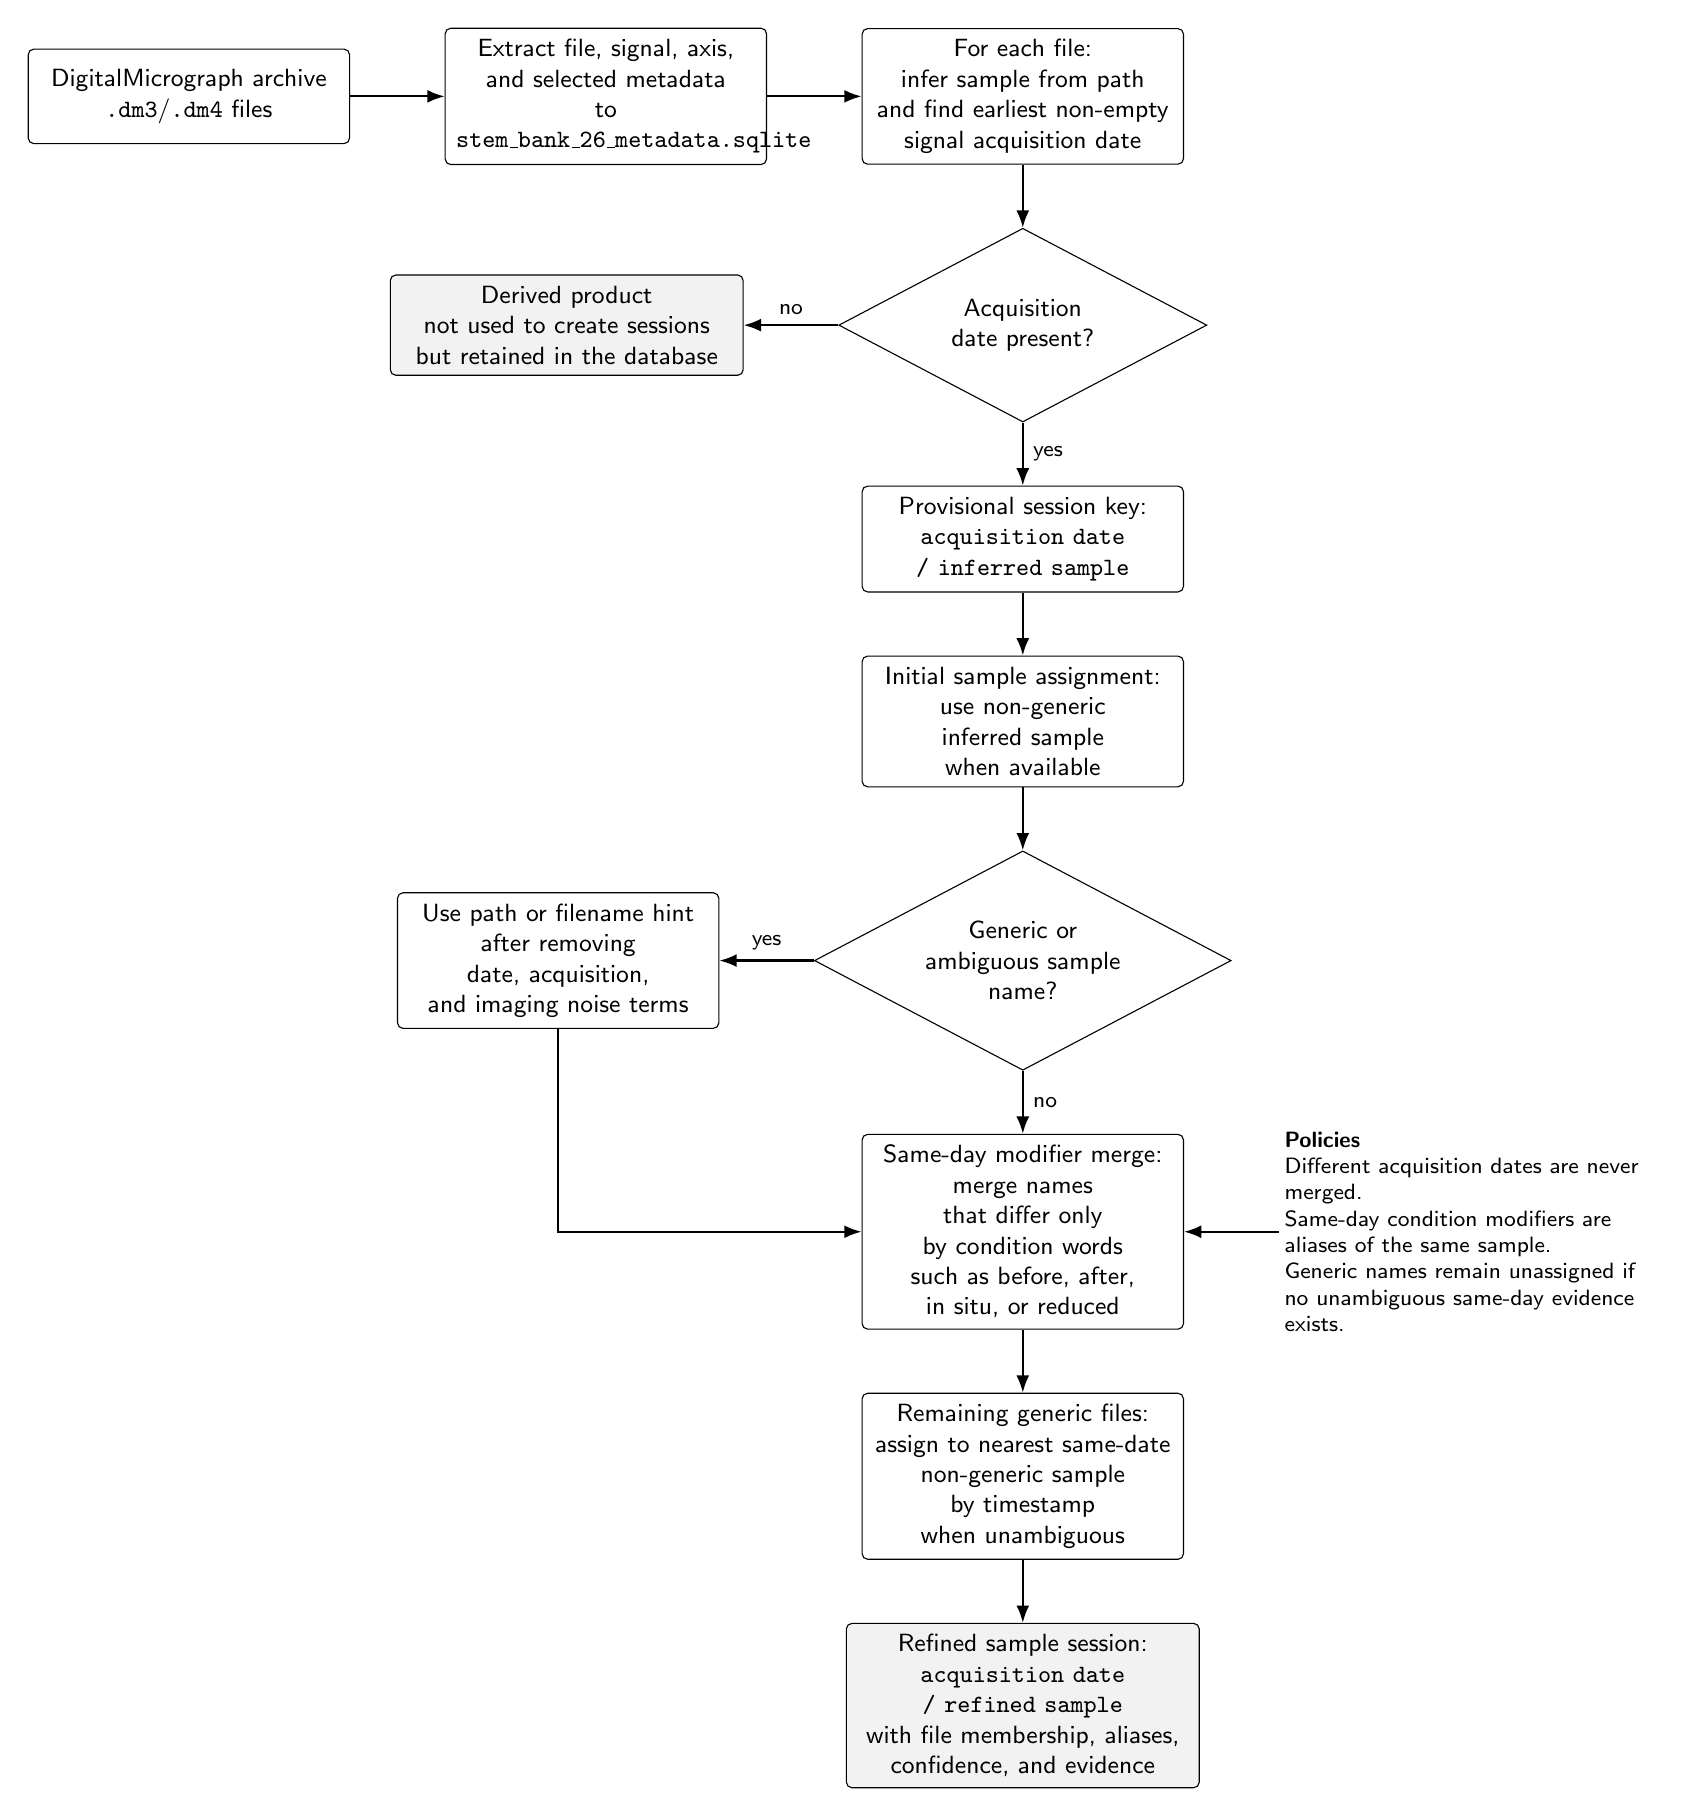
\begin{tikzpicture}[
    font=\sffamily\small,
    node distance=8mm and 12mm,
    flow/.style={-{Latex[length=2.2mm]}, thick},
    block/.style={
        draw,
        rounded corners=2pt,
        align=center,
        text width=38mm,
        minimum height=12mm,
        inner sep=4pt
    },
    decision/.style={
        draw,
        diamond,
        aspect=1.9,
        align=center,
        text width=31mm,
        inner sep=1.5pt
    },
    output/.style={
        draw,
        rounded corners=2pt,
        align=center,
        text width=42mm,
        minimum height=12mm,
        inner sep=4pt,
        fill=black!5
    },
    note/.style={
        align=left,
        text width=47mm,
        inner sep=2pt,
        font=\sffamily\footnotesize
    }
]

\node[block] (archive) {DigitalMicrograph archive\\
    \texttt{.dm3}/\texttt{.dm4} files};
\node[block, right=of archive] (metadata) {Extract file, signal, axis,\\
    and selected metadata\\
    to \texttt{stem\_bank\_26\_metadata.sqlite}};
\node[block, right=of metadata] (filelevel) {For each file:\\
    infer sample from path\\
    and find earliest non-empty\\
    signal acquisition date};

\node[decision, below=of filelevel] (hasdate) {Acquisition\\date present?};
\node[output, left=of hasdate] (derived) {Derived product\\
    not used to create sessions\\
    but retained in the database};
\node[block, below=of hasdate] (session) {Provisional session key:\\
    \texttt{acquisition date / inferred sample}};

\node[block, below=of session] (initialsample) {Initial sample assignment:\\
    use non-generic inferred sample\\
    when available};
\node[decision, below=of initialsample] (generic) {Generic or\\ambiguous sample\\name?};
\node[block, left=of generic] (hint) {Use path or filename hint\\
    after removing date, acquisition,\\
    and imaging noise terms};
\node[block, below=of generic] (modifier) {Same-day modifier merge:\\
    merge names that differ only\\
    by condition words\\
    such as before, after,\\
    in situ, or reduced};
\node[block, below=of modifier] (genericassign) {Remaining generic files:\\
    assign to nearest same-date\\
    non-generic sample\\
    by timestamp\\
    when unambiguous};
\node[output, below=of genericassign] (final) {Refined sample session:\\
    \texttt{acquisition date / refined sample}\\
    with file membership, aliases,\\
    confidence, and evidence};

\node[note, right=of modifier] (policy) {\textbf{Policies}\\
    Different acquisition dates are never merged.\\
    Same-day condition modifiers are aliases of the same sample.\\
    Generic names remain unassigned if no unambiguous same-day evidence exists.};

\draw[flow] (archive) -- (metadata);
\draw[flow] (metadata) -- (filelevel);
\draw[flow] (filelevel) -- (hasdate);
\draw[flow] (hasdate) -- node[above, font=\sffamily\footnotesize] {no} (derived);
\draw[flow] (hasdate) -- node[right, font=\sffamily\footnotesize] {yes} (session);
\draw[flow] (session) -- (initialsample);
\draw[flow] (initialsample) -- (generic);
\draw[flow] (generic) -- node[above, font=\sffamily\footnotesize] {yes} (hint);
\draw[flow] (hint) |- (modifier);
\draw[flow] (generic) -- node[right, font=\sffamily\footnotesize] {no} (modifier);
\draw[flow] (modifier) -- (genericassign);
\draw[flow] (genericassign) -- (final);
\draw[flow] (policy) -- (modifier);

\end{tikzpicture}
\end{document}
